\documentclass[12pt]{article}
\usepackage[margin=0.85in]{geometry}
\usepackage{amsmath,amssymb}
\usepackage{tikz}
\pagestyle{empty}
\setlength{\parindent}{0pt}
\setlength{\parskip}{3pt}

\newcommand{\q}[1]{\par\smallskip{\itshape #1}\par}

\begin{document}

\begin{center}
{\large Problem set 3 -- Econ 5030}
\end{center}

%%%%%%%%%%%%%%%%%%%%%%%%%%%%%%%%%%%%%%%%%%%%%%%%%%%%%%%%%%%%%%%%%%%%%%%
\textbf{1. Basic Cournot duopoly}
\q{Let begin by considering a Cournot duopoly. Each firm $i$ has the cost function $C(q_i)=cq_i^2/2$, where $c>0$. Market inverse $P(Q)=200-Q$.}

\q{\textbf{1.a} Write the profit of the arbitrary firm $i$.}
$\pi_i=(200-q_i-q_j)q_i-\tfrac{c}{2}q_i^2$.

\q{\textbf{1.b} Find the best response function for firm $i$ and graph it on the $q_i\times q_j$ plane.}
FOC $200-2q_i-q_j-cq_i=0\Rightarrow BR_i(q_j)=\dfrac{200-q_j}{2+c}$. Line from $(\tfrac{200}{2+c},0)$ to $(0,200)$ (graph below).

\q{\textbf{1.c} Find the Cournot equilibrium quantity $q^c$ and market price $p^c=P(2q^c)$.}
Symmetric: $q^c=\dfrac{200}{3+c}$, $p^c=\dfrac{200(1+c)}{3+c}$.

\q{\textbf{1.d} Graph the market outcome on the $p\times Q$ plane.}
Supply $=\sum MC$: $p=\tfrac{c}{2}Q$. Efficient $Q^*=\tfrac{400}{2+c}$, $p^*=\tfrac{200c}{2+c}$; Cournot at $(Q^c,p^c)$, $Q^c<Q^*$.

\begin{center}
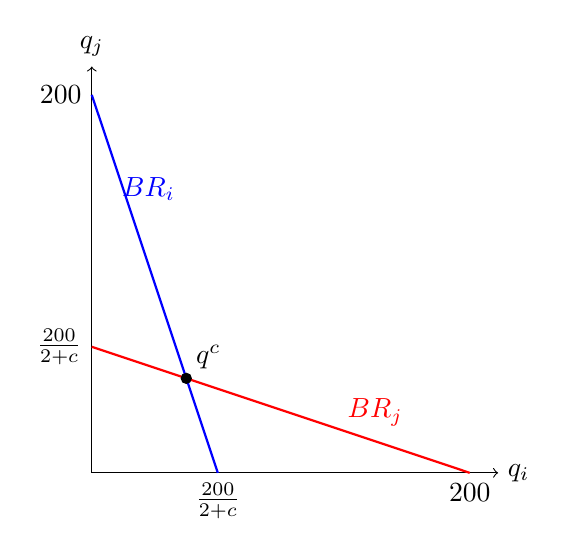
\begin{tikzpicture}[scale=0.024]
  \draw[->] (0,0) -- (215,0) node[right] {$q_i$};
  \draw[->] (0,0) -- (0,215) node[above] {$q_j$};
  \draw[thick,blue] (66.7,0) node[below,black] {$\frac{200}{2+c}$} -- (0,200) node[left,black] {$200$};
  \draw[thick,red] (0,66.7) node[left,black] {$\frac{200}{2+c}$} -- (200,0) node[below,black] {$200$};
  \fill (50,50) circle (3) node[above right] {$q^c$};
  \node[blue] at (30,150) {$BR_i$};
  \node[red] at (150,32) {$BR_j$};
\end{tikzpicture}
\qquad
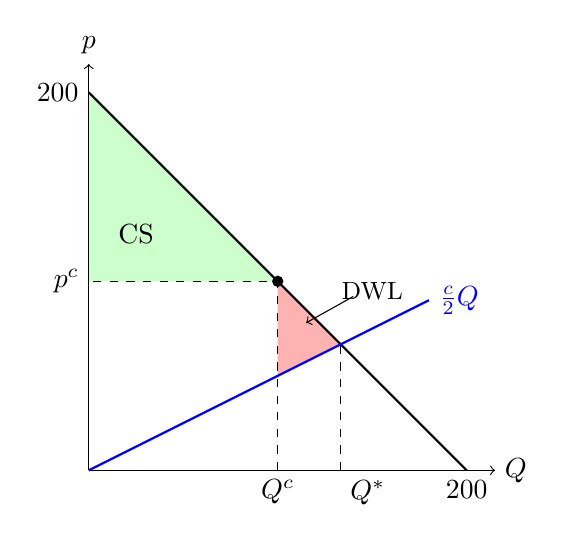
\begin{tikzpicture}[scale=0.024]
  \fill[green!20] (0,200) -- (0,100) -- (100,100) -- cycle;
  \fill[red!30] (100,100) -- (133.3,66.7) -- (100,50) -- cycle;
  \draw[->] (0,0) -- (215,0) node[right] {$Q$};
  \draw[->] (0,0) -- (0,215) node[above] {$p$};
  \draw[thick] (0,200) node[left] {$200$} -- (200,0) node[below] {$200$};
  \draw[thick,blue] (0,0) -- (180,90) node[right] {$\tfrac{c}{2}Q$};
  \draw[dashed] (100,0) node[below] {$Q^c$} -- (100,100) -- (0,100) node[left] {$p^c$};
  \draw[dashed] (133.3,0) node[below right] {$Q^*$} -- (133.3,66.7);
  \fill (100,100) circle (3);
  \node at (25,125) {CS};
  \node at (150,95) {\small DWL};
  \draw[->] (140,92) -- (115,78);
\end{tikzpicture}
\end{center}

\q{\textbf{1.e} Find an expression for the each firm's profits, the Consumer Surplus (CS), Total Surplus (TS) and Dead weight Loss (DWL).}
$\pi^c=q^c(p^c-\tfrac{c}{2}q^c)=\dfrac{20000(2+c)}{(3+c)^2}$,\quad $CS=\tfrac12(Q^c)^2=\dfrac{80000}{(3+c)^2}$,\quad $TS=CS+2\pi^c=\dfrac{40000(4+c)}{(3+c)^2}$.\\
$TS^*=\tfrac12\cdot200\cdot Q^*=\dfrac{40000}{2+c}$,\quad $DWL=TS^*-TS=\dfrac{40000}{(2+c)(3+c)^2}$.

%%%%%%%%%%%%%%%%%%%%%%%%%%%%%%%%%%%%%%%%%%%%%%%%%%%%%%%%%%%%%%%%%%%%%%%
\medskip
\textbf{2. Basic Cournot oligopoly}
\q{Let now consider a Cournot oligopoly with $n$ firms. Each firm $i$ has the cost function $C(q_i)=cq_i^2/2$, where $c>0$. Market inverse $P(Q)=200-Q$.}

\q{\textbf{2.a} Write the profit of the arbitrary firm $i$.}
$\pi_i=(200-q_i-Q_{-i})q_i-\tfrac{c}{2}q_i^2$.

\q{\textbf{2.b} Find the best response function for firm $i$ and graph it on the $q_i\times Q_{-i}$ plane.}
$BR_i(Q_{-i})=\dfrac{200-Q_{-i}}{2+c}$. Line from $(\tfrac{200}{2+c},0)$ to $(0,200)$; equilibrium where it meets $Q_{-i}=(n-1)q_i$ (graph below).

\q{\textbf{2.c} Find the Cournot equilibrium quantity $q^c$ and market price $p^c=P(nq^c)$.}
$(2+c)q^c=200-(n-1)q^c\Rightarrow q^c=\dfrac{200}{n+1+c}$, $p^c=\dfrac{200(1+c)}{n+1+c}$.

\q{\textbf{2.d} Graph the market outcome on the $p\times Q$ plane.}
Supply $p=\tfrac{c}{n}Q$; $Q^*=\tfrac{200n}{n+c}$; Cournot at $(Q^c,p^c)$ with $Q^c=\tfrac{200n}{n+1+c}<Q^*$.

\begin{center}
\begin{tikzpicture}[scale=0.024]
  \draw[->] (0,0) -- (215,0) node[right] {$q_i$};
  \draw[->] (0,0) -- (0,215) node[above] {$Q_{-i}$};
  \draw[thick,blue] (66.7,0) node[below,black] {$\frac{200}{2+c}$} -- (0,200) node[left,black] {$200$};
  \draw[dashed,gray] (0,0) -- (80,160) node[right,black] {\small $(n-1)q_i$};
  \fill (40,80) circle (3);
  \node[blue] at (30,165) {$BR_i$};
\end{tikzpicture}
\qquad
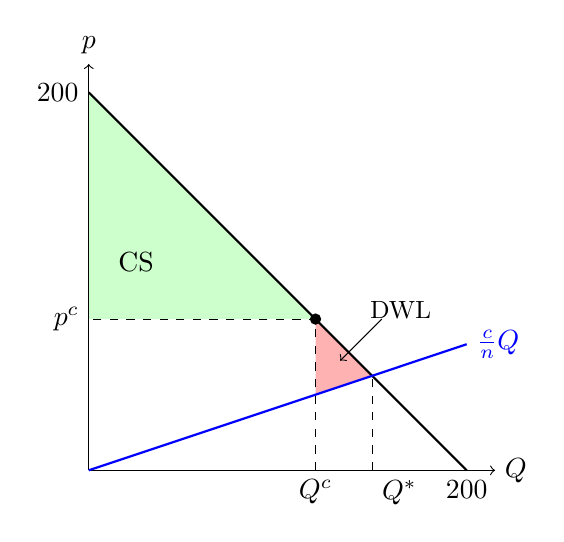
\begin{tikzpicture}[scale=0.024]
  \fill[green!20] (0,200) -- (0,80) -- (120,80) -- cycle;
  \fill[red!30] (120,80) -- (150,50) -- (120,40) -- cycle;
  \draw[->] (0,0) -- (215,0) node[right] {$Q$};
  \draw[->] (0,0) -- (0,215) node[above] {$p$};
  \draw[thick] (0,200) node[left] {$200$} -- (200,0) node[below] {$200$};
  \draw[thick,blue] (0,0) -- (200,66.7) node[right] {$\tfrac{c}{n}Q$};
  \draw[dashed] (120,0) node[below] {$Q^c$} -- (120,80) -- (0,80) node[left] {$p^c$};
  \draw[dashed] (150,0) node[below right] {$Q^*$} -- (150,50);
  \fill (120,80) circle (3);
  \node at (25,110) {CS};
  \node at (165,85) {\small DWL};
  \draw[->] (155,80) -- (133,58);
\end{tikzpicture}
\end{center}

\q{\textbf{2.e} Find an expression for the each firm's profits, the Consumer Surplus (CS), Total Surplus (TS) and Dead weight Loss (DWL).}
$\pi^c=\dfrac{20000(2+c)}{(n+1+c)^2}$,\quad $CS=\dfrac{20000n^2}{(n+1+c)^2}$,\quad $TS=\dfrac{20000n(n+2+c)}{(n+1+c)^2}$.\\
$TS^*=\dfrac{20000n}{n+c}$,\quad $DWL=\dfrac{20000n}{(n+c)(n+1+c)^2}\to0$ as $n\to\infty$.

%%%%%%%%%%%%%%%%%%%%%%%%%%%%%%%%%%%%%%%%%%%%%%%%%%%%%%%%%%%%%%%%%%%%%%%
\medskip
\textbf{3. Cournot with Product Differentiation}
\q{Take the inverse demand system: $P_1(q_1,q_2)=18-q_1-\gamma q_2$, $P_2(q_2,q_1)=18-q_2-\gamma q_1$. Assume both firms have NO COST of production. Now let us look at the Cournot solution for general $\gamma$ between zero an one.}

\q{\textbf{2.a} Write out each firm's profit function and label them $\Pi_1(\gamma)$ and $\Pi_2(\gamma)$.}
$\Pi_1(\gamma)=(18-q_1-\gamma q_2)q_1$,\quad $\Pi_2(\gamma)=(18-q_2-\gamma q_1)q_2$.

\q{\textbf{2.b} Find each firm's best response function by solving $\frac{\partial\Pi_1(\gamma)}{\partial q_1}=0$ for $q_1^\gamma(q_2)$ and $\frac{\partial\Pi_2(\gamma_2,\gamma_1)}{\partial q_2}=0$ for $q_2^\gamma(q_1)$.}
$18-2q_1-\gamma q_2=0\Rightarrow q_1^\gamma(q_2)=\dfrac{18-\gamma q_2}{2}$;\quad $q_2^\gamma(q_1)=\dfrac{18-\gamma q_1}{2}$.

\q{\textbf{2.c} Graph the best response functions of the firms' on $q_1\times q_2$ space.}
\begin{center}
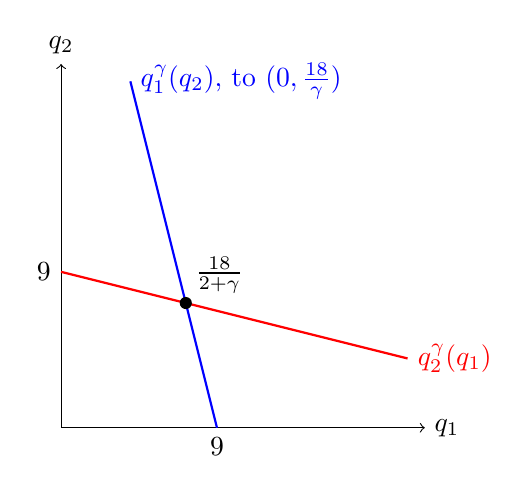
\begin{tikzpicture}[scale=0.22]
  \draw[->] (0,0) -- (21,0) node[right] {$q_1$};
  \draw[->] (0,0) -- (0,21) node[above] {$q_2$};
  \draw[thick,blue] (9,0) node[below,black] {$9$} -- (4,20) node[right] {$q_1^\gamma(q_2)$, to $(0,\frac{18}{\gamma})$};
  \draw[thick,red] (0,9) node[left,black] {$9$} -- (20,4) node[right] {$q_2^\gamma(q_1)$};
  \fill (7.2,7.2) circle (0.35) node[above right] {$\frac{18}{2+\gamma}$};
\end{tikzpicture}
\end{center}

\q{\textbf{2.d} Find the equilibrium quantities and prices and label them $q_1(\gamma)$, $p_1(\gamma)$ and $q_2(\gamma)$, $p_2(\gamma)$.}
$q_1(\gamma)=q_2(\gamma)=\dfrac{18}{2+\gamma}$,\quad $p_1(\gamma)=p_2(\gamma)=\dfrac{18}{2+\gamma}$ \quad ($\Pi_i=\tfrac{324}{(2+\gamma)^2}$).

%%%%%%%%%%%%%%%%%%%%%%%%%%%%%%%%%%%%%%%%%%%%%%%%%%%%%%%%%%%%%%%%%%%%%%%
\medskip
\textbf{4. Price competition}
\q{Suppose that thre are 2 firms in a Bertrand oligopoly with homogenous products. Each firm $i$ has th cost of production $c(q_i)=q_i^2/2$. The industry demand function is the rectangle $D(p)=0$ if $p>10$, $D(p)=10$ if $p\le10$. The if firms price the same then demand is split evenly. Each firm $i$ has th cost of production $c(q_i)=q_i^2/2$. Based on this cost structure a firm will never supply more than their supply function $s(p_i)=p_i$. using this fact we can construct residual demand and firm profit. Firm profit is the piecewise function for prices in the interval $[0,10]$ (I have done all the work for you here):
\[
\pi_i(p_i,p_j)=\begin{cases}
p_i\min\{p_i,10-p_j\}-\big(\min\{p_i,10-p_j\}\big)^2/2 & p_i>p_j\\
p_i5-12.5 & p_i=p_j>5\\
p_i^2/2 & p_i=p_j\le5\\
p_i^2/2 & p_i<p_j
\end{cases}
\]}

\q{\textbf{1.} Because for most prices $p_j$ the best response is not well-defined, instead find the argument of the supremum of the profit responding to the other firm's price. Formally find $\phi(p_j)=\arg\sup_{p_i\in[0,10]}\pi_i(p_i,p_j)$.}
Undercut: $\sup=p_j^2/2$ (not attained). Match: $\le p_j^2/2$ (for $p_j>5$, $p_j^2/2-(5p_j-12.5)=\tfrac12(p_j-5)^2>0$). High: increasing in $p_i$, so $p_i=10$, giving $10(10-p_j)-\tfrac12(10-p_j)^2=\tfrac{100-p_j^2}{2}$. High $\ge$ undercut iff $p_j\le5\sqrt2$:
\[
\phi(p_j)=10 \text{ for } p_j\le5\sqrt2;\qquad \phi(p_j)=p_j^- \text{ (just below } p_j\text{, not attained) for } p_j>5\sqrt2.
\]

\q{\textbf{2.} Make a formal argument that symmetric prices cannot be a pure strategy Nash equilibrium.}
$p_1=p_2=p\le5$: earn $p^2/2\le12.5$; deviate to 10: $\tfrac{100-p^2}{2}\ge37.5$. $p>5$: earn $5p-12.5$; deviate to $p-\varepsilon$: $\to p^2/2>5p-12.5$. Profitable deviation either way.

\q{\textbf{3.} Make a formal argument that asymmetric prices cannot be a pure strategy Nash equilibrium.}
$p_j<p_i$: $j$ earns $p_j^2/2$; any $p_j'\in(p_j,p_i)$ still undercuts and earns $p_j'^2/2>p_j^2/2$. Profitable deviation.

\q{\textbf{4.} Use your result from 1 to find the bound of best response prices.}
Best responses lie in $[5\sqrt2,\,10]\approx[7.07,10]$; upper bound $\bar p=10$.

\q{\textbf{5.} Solve for the mixed strategy equilibrium using pricing bounds using the answer to 1.}
Symmetric CDF $F$ on $[\underline p,10]$, no atoms (tie earns $5p-12.5<p^2/2$, so mass is undercut). At $\underline p$ always lowest: $k=\underline p^2/2$. At $10$ always highest: $k=E[(100-X^2)/2]$. So $E[X^2]=100-\underline p^2$; $\underline p=5\sqrt2$ would force an atom, so $\underline p<5\sqrt2$.

\q{\textbf{6.} Solve for the Nash Equilibrium Mixed strategies.}
Indifference on $[\underline p,10]$ (high firm sells $10-x$):
$\int_{\underline p}^{p}[p(10-x)-\tfrac12(10-x)^2]dF(x)+(1-F(p))\tfrac{p^2}{2}=k$.
Differentiating twice, $S=1-F$, $t=p-5$: $2t^2S''+6tS'+S=0$, roots $r=-1\pm\tfrac{1}{\sqrt2}$. With $F(10)=1$:
\[
F(p)=1-C\big[5^{\sqrt2}(p-5)^{-1-1/\sqrt2}-(p-5)^{-1+1/\sqrt2}\big],\quad p\in[\underline p,10],
\]
with $F(\underline p)=0$ and $\underline p=2(\underline p-5)^2f(\underline p)$ giving $\underline p\approx6.60$, $C\approx0.287$.

\q{\textbf{7.} Calculate the Nash equilibrium expected profits.}
$E[\pi_i]=\underline p^2/2\approx21.8$ per firm.

\end{document}
